%%% DOCUMENT SETUP %%%
\documentclass{llncs}
\usepackage[greek,english]{babel}

%%% LAYOUT %%%
\usepackage{fullpage}
\usepackage[parfill]{parskip}
\usepackage{multicol}
\usepackage{footnote}

%%% GRAPHICS %%%
\usepackage{graphicx}
\usepackage{color}
\usepackage{graphics}
\usepackage{rotating}
\usepackage{subfig}
\usepackage{amsmath}
\usepackage{amssymb}
\usepackage{amscd}
% \usepackage{xfrac}
\usepackage{float}
\usepackage{dsfont}
\graphicspath{{./figures/}}

%%% FONT %%%
\usepackage{ifxetex}
\ifxetex
  \usepackage{fontspec}
    \setmainfont{Linux Libertine O}
  \usepackage{xunicode}
  \usepackage{microtype}
\else
  \usepackage[T1]{fontenc}
  \usepackage[latin1]{inputenc}
  \usepackage{times}
  \usepackage{microtype}
\fi

%%% Coding %%%
\usepackage{listings}
\usepackage{algpseudocode}
\usepackage{algorithm}

%%% TITLE PAGE %%%
\author{Jeroen Hofman (jhn343) \ \ \ \ \ John Tyree (jte320)
\institute{Vrije Universiteit}}
\title{Data Mining Techniques\\
    Assignment 3}

\begin{document}
\maketitle
\captionsetup{width=0.8\textwidth}
\thispagestyle{empty}

%% %%% ABSTRACT %%%
%% \begin{center}
%% \begin{abstract}
%% \end{abstract}
%% \end{center}

%%% TABLE OF CONTENTS %%%
\newpage
% \tableofcontents
% \newpage

\section{Introduction}
In this last assignment we try to predict the outcomes of soccer matches using historical data starting from 2002. Before we try to make actual predictions, we do some exploration of the data-set. We then proceed by building a model consisting of two parts. First we built from the data a ranking list of all the teams, then we use this ranking list to generate probability density functions for the outcome of a match based on rank differences between teams. We used a number of different approaches for generating these PDFs. Finally we use this model on 114 matches of which the outcome is assumed to be unknown, from which a score is calculated.

\section{Exploratory Data Analysis}
For the assignment we are given a CSV file named 'FIFA0212.csv' consisting of 9302 entries of matches played from 01/01/2002 up to 30/06/2012. Up to 18/05/2012 the outcomes of the matches are known. We are supposed to use these data up to 18/05/2012 to model the outcomes and use this model to predict 114 soccer matches from 18/05/2012 up to and including 05/06/2012. The attributes of the entries are 'Date', `Team1', 'Team2', 'Score1', 'Score2', 'HomeTeam', 'ET', 'PSO', 'Location', 'Type' and 'Info'. There are a few teams that appear in the list but who are not quoted by the FIFA ranking list \cite{FIFAranking} today, these are 'Yugoslavia', 'Serbia and Montenegro' and 'Netherlands Antilles', hence we removed these entries from the data. After some consideration we decided to focus on only a few attributes, namely 'Date', 'Team1', 'Team2', 'Score1', 'Score2', 'HomeTeam'. Since for the assignment we are only interested in probabilities of winning/losing/tying and not in the actual scores, we added an attribute 'Outcome', with the following simple rules:

\begin{equation*}
  \text{Outcome} =
  \begin{cases}
    1, & \text{if Score1 > Score2} \\
    0.5, & \text{if Score1 = Score2} \\
    0, & \text{if Score1 < Score2}
  \end{cases}
\end{equation*}

Figure \ref{fig:ex} shows an example of the data we are working with. The extra attribute 'Weight' will be explained in the next section. The number of matches we can use to predict, when having applied the above filters, is 9016. On these entries we can do some additional exploratory analysis. From these 9016 matches 23.8\% resulted in a tie, 48.4\% resulted in a win for Team1 and 27.8\% resulted in a loss for Team2. The reason that these last two numbers are not roughly equal is the home-team advantage. If the home-team attribute is 1 then Team1 is a home-team, otherwise none of the teams is a home-team. If we look at only home-team matches we find that Team1 wins in 50.3\% of the cases, while if we look at normal matches Team1 only wins in 42.7\% of the cases, which is a significant difference.

\begin{figure}
  \centering
  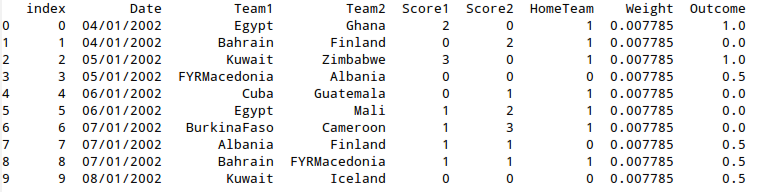
\includegraphics[width=1.0\textwidth]{ex.png}
  \caption{Example of the data-set.}
  \label{fig:ex}
\end{figure}

We can also look at how much data we actually have. All 208 countries currently in the FIFA ranking list are present in the list of matches. That means that on average each team has played (9016*2)/208 $\approx$ 87 matches, which is a significantly large number. Even small (soccer-wise unimportant) countries like Fiji or The Seychelles have 30-50 entries. The country with the smallest number of entries in the data set is Sao Tom\'e en Principe with 8 entries. The country with the largest number is Bahrain with 185 matches.

\section{Model}
The algorithm we have used consists of 3 parts, which will be discussed in detail below. First, we use a modified version of a model called Elo++ to generate a ranking table for all the participating teams. Then we use these ranking table to determine probability density functions (PDFs) of winning/losing/tying based on rank differences between teams. Thirdly we use these PDFs to make predictions on outcomes of matches.

\subsection{Ranking}
The first part of our algorithm consists of a modified version of a method called Elo++. The method is based on a paper written by the winners of a data mining competition on Kaggle.com where they were given a detest of historical chess games with outcomes and were asked to predict the outcomes of future games \cite{Sismanis}. Due to the similar structure of this problem and our problem we decided to use this paper as a starting point for our model. Since the justification of parts of the model can be found in \cite{Sismanis}, we will mainly focus on our interpretation.

Since matches played in 2002 are less relevant than matches played in, say, 2010, we want to give different weights to matches according to their times tamp. Following the paper we use the following weighting scheme:

\begin{equation*}
    w_{ij} = \left(\frac{1 + t_{ij} + t_{\text{min}}}{1 + t_{\text{max}} - t_{\text{min}}}\right)^{\gamma}
\end{equation*}

where $w_{ij}$ is the weight of a match between team $i$ and team $j$, $t_{\text{min}}$ is the time the first match was played, $t_{\text{max}}$ is the time when the last match was played, $t_{ij}$ is the time when the match was played for which we are calculating the weight, and $\gamma$ is a model parameter determining the shape of the weighting function. We counted the time in years, so that January 2002 corresponds to $t = 1/12$ and May 2012 corresponds to $t = 10 \; 5/12$. The steepness of the curve is controlled by $\gamma$, named \emph{factor} in our program. Some test results are given in the next section.

Using this weighting function and the outcome attribute $o_{ij}$ ($i$ being Team1 and $j$ being Team2) we introduced in the previous section, we can implement a stochastic gradient descent technique, of which the pseudo-code is shown below:

\begin{algorithm}[H]
\caption{Stochastic gradient descent method.}
\begin{algorithmic}
\Require {T: training data-set, P: total number of iterations} \\
for all players $i, r_i\gets 0$ \\
for all games in T compute weights $w_{ij}$ (see above)
\For {$p=1 \; \bold{to} \; P$}
\State $\eta \gets ((1 + 0.1P)/(p + 0.1P))^{0.602}$
    \ForAll {\emph{shuffled} tuples $<i,j,t_{ij},o_{ij}>$ in T}
    \State $\hat{o}_{ij} = 1/(1 + \exp{r_j - r_i})$
    \State $r_i \gets r_i - \eta(w_{ij}(\hat{o}_{ij} - o_{ij})\hat{o}_{ij}(1 - \hat{o}_{ij}))$
    \State $r_j \gets r_j - \eta(-w_{ij}(\hat{o}_{ij} - o_{ij})\hat{o}_{ij}(1 - \hat{o}_{ij}))$
    \EndFor
\EndFor \\
\Return all ratings $r_i$
\end{algorithmic}
\label{alg:1}
\end{algorithm}

The algorithm is substantially different from the one in the paper since the authors include neighborhoods of chess players, since in chess high-ranked players only play against other high-ranked players. This is however not the case for soccer matches and hence we skip the whole part about neighborhoods, thereby simplifying the algorithm. In the algorithm we compute the weights for all matches, then we do an iteration, where each iteration we loop over all the matches in the training data-set in a shuffled manner. The algorithm then compares the predicted outcome based on ranks $\hat{o}_{ij}$ and compares this with the actual outcome of the match and adjusts the rankings accordingly (if $\hat{o}_{ij} = o_{ij}$ the ranks are unchanged). Due to the learning rate $\eta$ the rankings will shift significantly in the beginning but are forced to converge when $p \rightarrow P$.

The free parameter in this model is the number of iterations $P$, in our model referred to as the variable \emph{iter}. We will give some results for various values of \emph{iter} in the next section. In the paper they mention convergence after $P = 50$, however it is unclear what is meant by this, since convergence will always occur due to the learning rate.

We can test the results from this part of the model by comparing by the ranking list provided by FIFA. They use a different algorithm for computing the ranking \cite{FIFAcalc}, but the results should be similar. Figure \ref{fig:rank} below shows the results of our ranking for the 20 highest ranked countries, where the training set is the complete data set prior to 18/05/2012, with $gamma = 1$ and \emph{iter} = 300. The left figure shows our results, the right figure the results from FIFA obtained from \cite{FIFAranking}. The figures are not the same, however most names occur in both lists, showing that our model gives still a fairly accurate prediction.

\begin{figure}
  \centering
  \subfloat{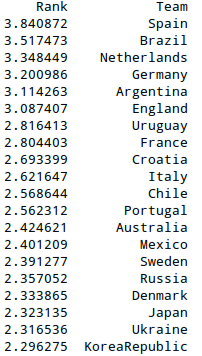
\includegraphics[width=0.3\textwidth]{model_ranking.png}}
  \subfloat{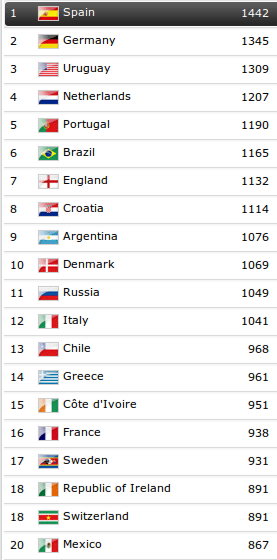
\includegraphics[width=0.3\textwidth]{rank_fifa.png}}
  \caption{The 20 highest ranked countries, according to our model (left) and according to FIFA (right).}
  \label{fig:rank}
\end{figure}

\subsection{Probability Density Functions}

In the previous section we described the algorithm to obtain a ranking for all teams in the data-set. We use these ranking per team to calculate a rank difference for each match in the training set. The rank difference is based upon the actual ranking numbers produced by the model in the previous section, not on the stylized integer ranking, so for instance if Spain plays against Germany, that match would have a ranking difference of 3.84 - 3.20 = 0.64, i.e. the rank of Team1 minus the rank of Team2. Note that this number can be negative as well. A crucial assumption we make for the next steps in our model is that there is no difference in behavior for matches with the same rank difference, i.e. a match of Germany and Spain (rank difference 0.64) will follow the same statistics for predicting the outcome (see below) as a match between the Cayman Islands and Bhutan (rank difference 0.66) because their rank differences are nearly the same.

We make a set of histograms as a function of rank difference, one for winning a game, one for tying a game and one for losing a game. By looping over all the matches in the training data-set, we calculate for each match the rank difference (rank Team1 - rank Team2), look at the outcome and add a count to the appropriate histogram (dependent on the outcome) in the appropriate bin (dependent on the rank difference). In this way we obtain three histograms, which have to be normalized with respect to each other to give the probability that a match with a given rank difference will end in a win, tie or loss from the perspective of Team1. An important parameter related to generating these histograms is the bin width, the variable \emph{bin\_width} in our model. We tried several settings for this parameter, more on that in the next section. We tried different approaches regarding the generation of histograms:

\begin{itemize}
  \item
    The approach as described above: Calculate the rank difference for each match from the perspective of Team1, look up the outcome and add a count to the appropriate histogram in the appropriate bin.
  \item
    The same as above but with home-team advantage built in: Calculate the rank difference for each match from the perspective of Team1, look up the outcome, look up whether Team1 is a home-team or not and construct a desperate set of histograms for the home-team cases. Hence we have 6 histograms in this case.
  \item
    The same approaches as the two above, but now as seen from the highest ranked player, this will prevent the rank difference from being negative and hence increase the amount of statistics we have. However, if we take home-teams into account, we lose information on which team is a home-team and so we have to construct for the second case 9 histograms, 3 for no home-team, 3 for the highest ranked player being a home-team and 3 for playing against a home-team.
  \item
    A last improvement we implemented is fitting functions to these histograms to remove statistical noise and anomalies.
\end{itemize}

Figure \ref{fig:hist} gives an example of the last 2 cases mentioned above for \emph{bin\_width} = 0.1. The figures below give the probabilities of winning (green), tying (blue) and losing (red) as a function of rank difference as seen from the highest ranked player. The left figure gives the results when no home-team is involved, the figure in the middle gives the results for the highest ranked player being a home-team and the right figure gives the results for playing against a home-team.

\begin{figure}[h]
  \centering
  \subfloat{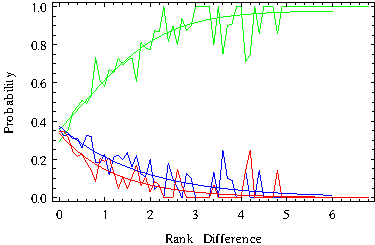
\includegraphics[width=0.33\textwidth]{nohome.pdf}}
  \subfloat{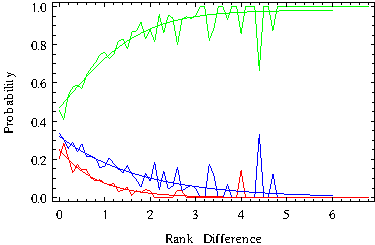
\includegraphics[width=0.33\textwidth]{home.pdf}}
  \subfloat{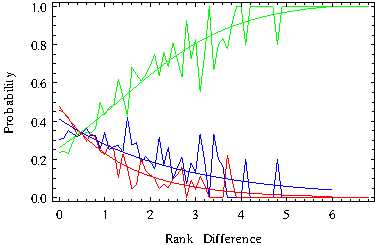
\includegraphics[width=0.33\textwidth]{ahome.pdf}}
  \caption{Probability density functions including fits for winning, tying and losing a game as seen from the highest ranked player for no home-team (left), the highest ranked being a home-team (middle) and against a home-team (right).}
  \label{fig:hist}
\end{figure}

The probability of winning is almost always the highest, since we are looking from the perspective of the highest ranked player. This is not the case when playing against a home-team while the rank difference is lower, as is expected. The probability to win is higher when the player is playing as a home-team then when it is not. From the data it is clear that there is some substantial noise, because of the peaks in the data. The straight lines are simple exponential fits which smoothen out these effects.

\subsection{Prediction}
The last step in the model is going from the PDFs based on rank differences to an actual prediction for a match with unknown outcome. The most straightforward way is to look at a new match, compute the rank difference between the two teams, then look up the appropriate bin in the histogram corresponding to the rank difference, possibly taking into account if one of the teams is a home-team (which boils down to choosing different sets of histograms). Then from either the histograms or the fitted functions obtain the probabilities for the highest ranked to win, tie or loose and use these probabilities directly for the prediction. As an example, we look at a match  on 23/07/2009 of the USA against Honduras, in which the rank difference, as seen form the USA, is 0.71. The USA was also a home-team in this match. If we want to take into account home-team advantages we look at the fits of the tuple of histograms corresponding to the highest ranked player being a home-team, in this case we get P(win) = 0.66, P(tie) = 0.24, P(loss) = 0.10.

There is however also the possibility of assigning 1 point to the most probable outcome and 0 to the other outcomes. This will however mean, using figure \ref{fig:hist}, the prediction will almost always be that winning is the most probable outcome (the green line is almost always higher than the other two lines).

A comparison between these two methods (and some other) will be made in the next section where the results are discussed using cross-validation.

\section{Results}

\subsection{Cross Validation}
To evaluate the quality of the model, we used an adapted cross-validation technique, under the assumption that predicting past games from future data was not truly indicative of model performance in the context of the competition. To avoid this issue, we turned to a rolling validation scheme where the model was trained on a fixed length window of $N$, matches and then applied to predict the outcome of the following $N$ matches.

\subsection{Parameter Optimization}
Having developed a reasonable looking model that was capable of replicating the expected results (Fig.~\ref{fig:rank}), we now had to find the optimal values for the three models' parameters: $\gamma$, \emph{iter} and \emph{bin\_width}.

Our first step was to explore the behavior of the ranking model parameters, in order to build a solid foundation open which to test our prediction techniques. Choosing a simple value of $\gamma = 1.5$, based on the intuition that more recent games should be more influential, we varied the number of iterations performed during the training phase. The results are presented in table~\ref{tab:iter}. We see that after approximately 100 iterations, the ranking system stabilizes enough that scores become consistent. Therefore, we took a value of $iter = 150$ to be sufficient for testing purposes, with more detailed analysis delayed until later.

We next trained the model using a wide range of values for $\gamma$, from 0 (all games have equal weight), to 3 (cubic decay). In this case (table~\ref{tab:factor}), it is apparent that our original intuition about the relative importance of recent matches compared to old matches was probably correct, although still not very powerful. A value which is two high also proves problematic however, likely  due that the fact that it penalizes older matches so heavily that it is analogous to not having them at all. From this, it follows generally that less training data leads to weaker predictive power. We chose a value of $\gamma = 1.5$ as it was the best performing and also a somewhat ``average'' value.

Having selected a value for $\gamma$, we revisited our selection of $iter$. Figure~\ref{fig:rankconvergence}, shows the changing distribution of the ranks throughout the training process, for different values of the learning rate $\eta$. We don't treat $\eta$ as a free parameter, but we wanted to make sure that our rank distribution was stabilizing naturally and not simply because we were forcing it by taking $\eta \to 0$. Figure~\ref{fig:ranknolearn}, shows that the ranks do indeed remain relatively stable after a period, even without the help of a low $\eta$ value. It was also clear however, that there were a few sporadic cases of teams with low ranks being quite slow to descend out of the pack. To combat this, we allowed the simulation to run indefinitely, stopping when the absolute ordering of team ranks stabilized. This occurred around 300 iterations, as shown in figure~\ref{fig:ranklearn300}.

These two parameters, $iter$ and $\gamma$, are only relevant to the ranking algorithm. Having decided on reasonable values of $iter = 300$ and $\gamma = 1.5$, we next examined the histogram based generation of PDFs as described previously. Here, the parameter to optimize was the width, in terms of rank difference, of a bin in the histogram. We varied this from 0.01 up to 10, which translates to 1000 bins, down to a single bin. Table~\ref{tab:binwidth} illustrates again that extreme values tend to perform poorly compared to more moderate choices. In the case of bin width 2, we are beginning to effectively ignore the rank difference entirely. Conversely, taking bin width 0.01 potentially poses a significant threat of over fitting the data, but this is largely mitigated by our decision to model the histograms with monotonic exponential functions (fig.~\ref{fig:hist}).

\subsection{Prediction Confidence}

We felt that, in theory, the generation of PDFs from the data using the histogram method would provide the most optimal confidence metric for predicting game outcomes. It was only in the spirit of validating this assumption that we tested alternate confidence determining algorithms. Here we compare our PDF method with two much simpler methods. In the first method, we simply select the most likely victor based on the likelihoods given by the PDF functions. For example, if we predict a 40\% chance that Team1 wins a match, 30\% to tie, and 30\% to lose, then we declare with 100\% confidence that Team1 will win this match and the model outputs ``1,0,0''. We call this model the ``All-Or-Nothing'' approach. This model is good in the sense that it is, in fact, the \emph{only} way to achieve a perfect score, but assuming that sometimes we make incorrect predictions, we expected this method to perform poorly overall. The results in table~\ref{tab:performance} clearly indicate otherwise.

After discovering that the All-Or-Nothing approach was superior to our carefully crafted PDF predictions, we tried a second model, referred to as the ``80-20'' model. In this model, we assign 80\% confidence to the most likely outcome as given by the PDF, and 20\% to the ``neighboring'' outcome. For example, if Team1 is predicted to win, the model will output ``0.8, 0.2, 0''. Similarly, if a tie is predicted, the output will be ``0.1, 0.8, 0.1''. Again, table~\ref{tab:performance} shows that the All-Or-Nothing approach is superior to this one in every tested situation.

At first this was disappointing, but some further analysis reveals the likely cause. By assuming that the scores should given by each method should be roughly the same in expectation, we were implicitly assuming that the PDF output was symmetric, that is, the median probability would be ``0.33, 0.33, 0.33''. In reality, after considering home-team advantage and the fact that tie matches occur more infrequently than random chance would suggest, we find a median probability of roughly ``0.6, 0.15, 0.25''. If we treat this as an optimization problem such that
\begin{align*}
    P(a,b,c) = 0.6*a + 0.15*b + 0.25*c,
\end{align*}
$P(1,0,0)$ is the obvious solution, giving a score of 0.6 (which
is indeed what we find).

\begin{figure}
    \begin{center}
        \subfloat[Constant Learning Rate]{
        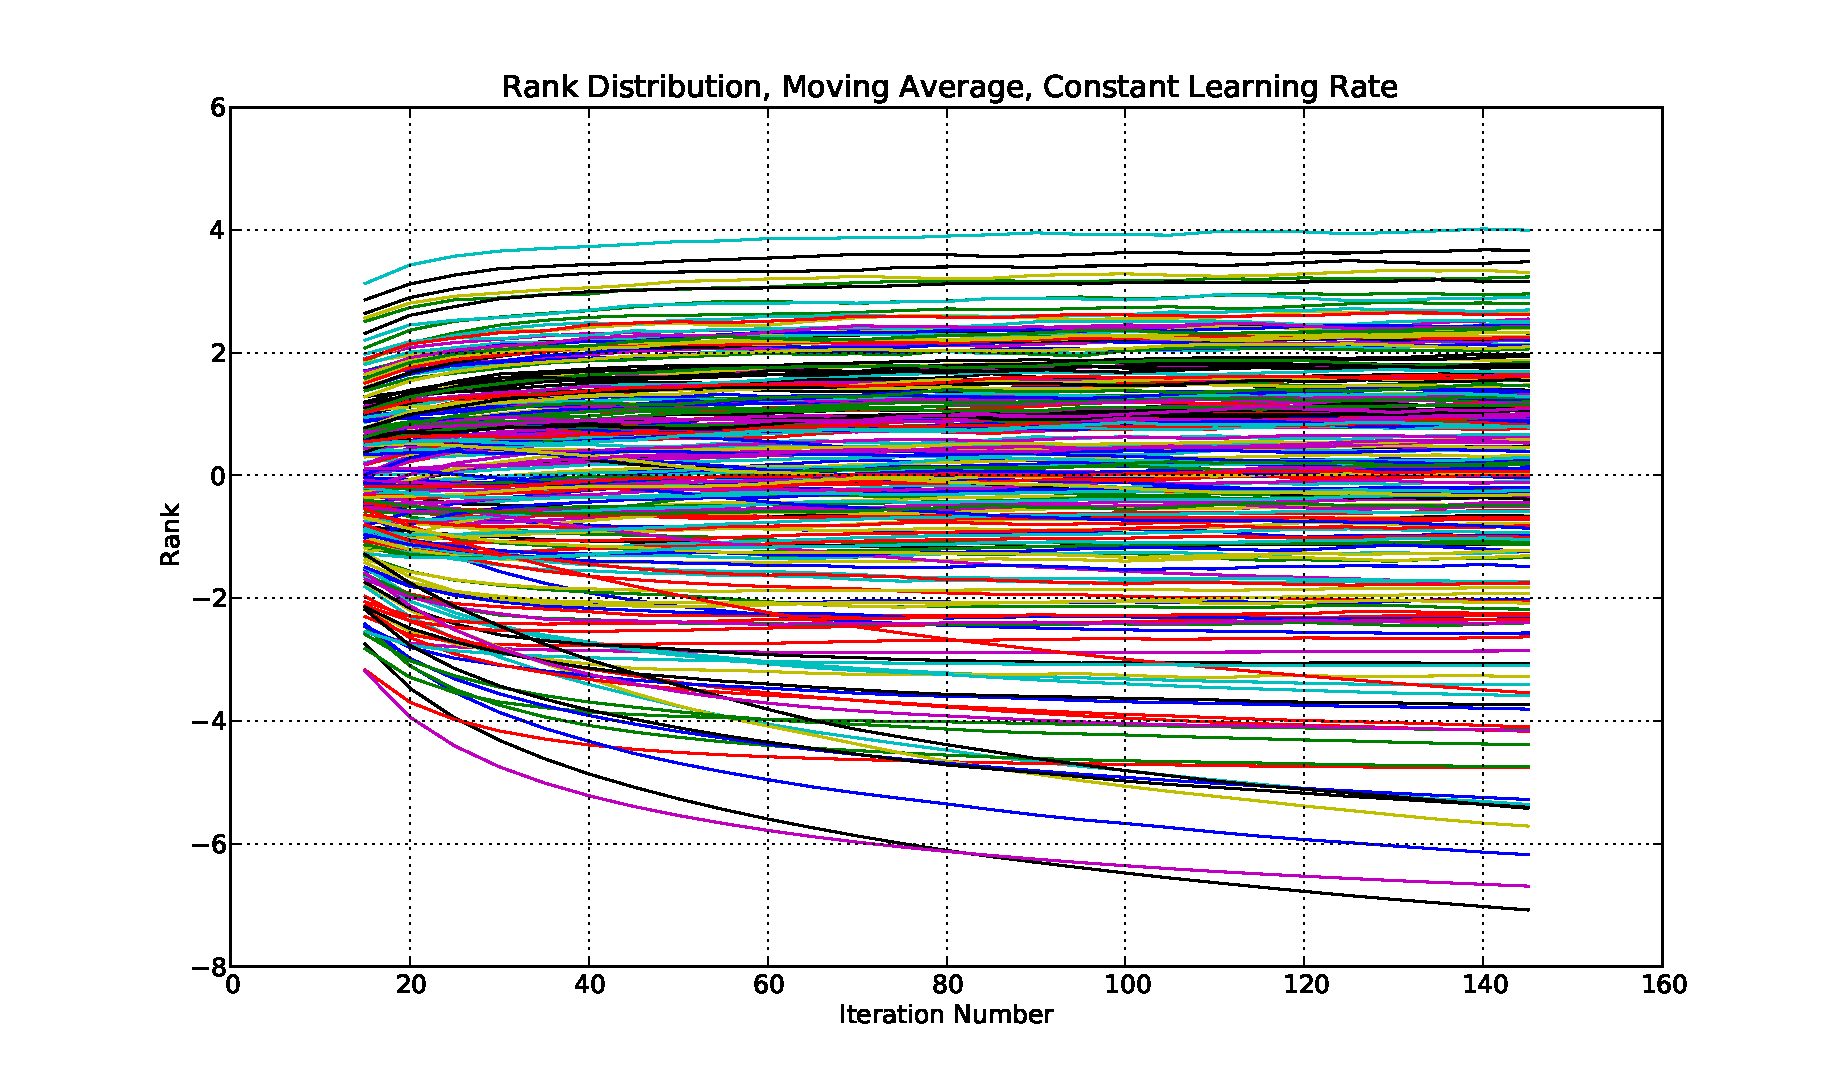
\includegraphics[width=0.45\linewidth]{RankMovAvgNoLearn.pdf}
        \label{fig:ranknolearn}
        }
        \subfloat[Linear Decay Learning Rate]{
        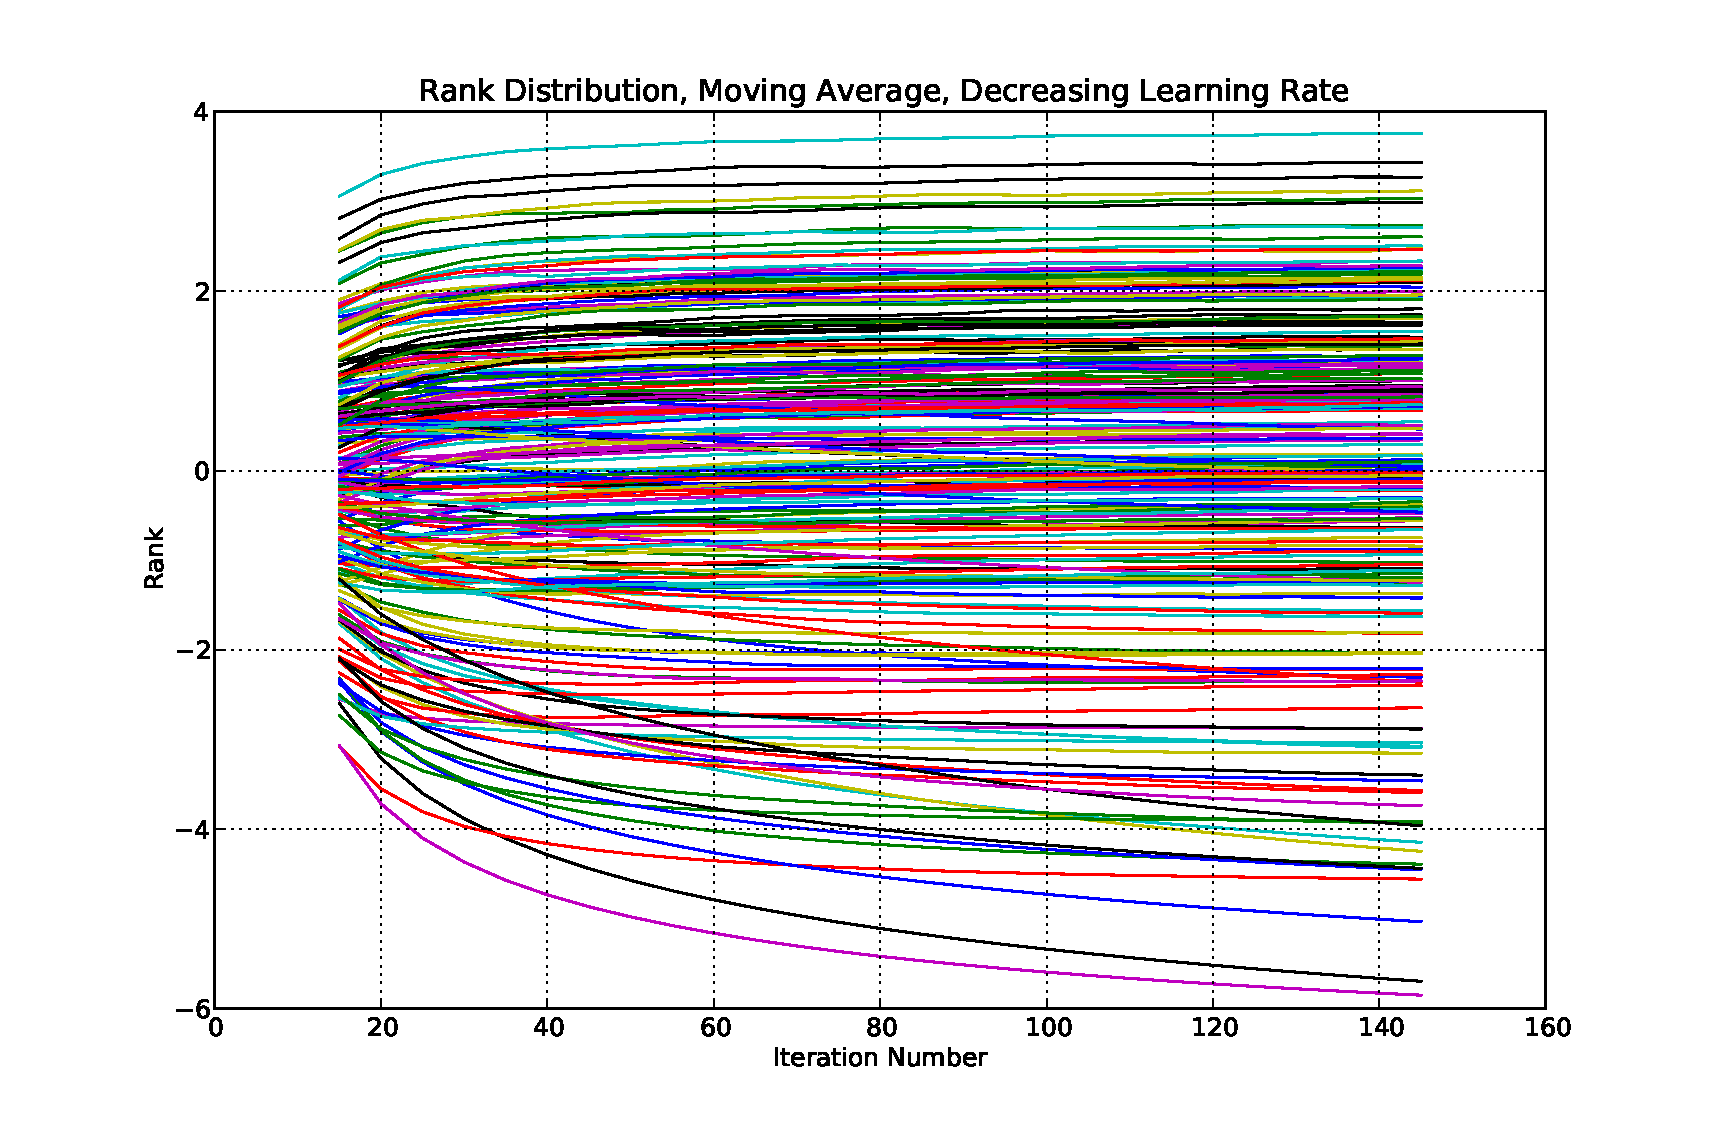
\includegraphics[width=0.45\linewidth]{RankMovAvgLearn.pdf}
        \label{fig:ranklearn}
        }\\
        \subfloat[Iteration until Convergence]{
        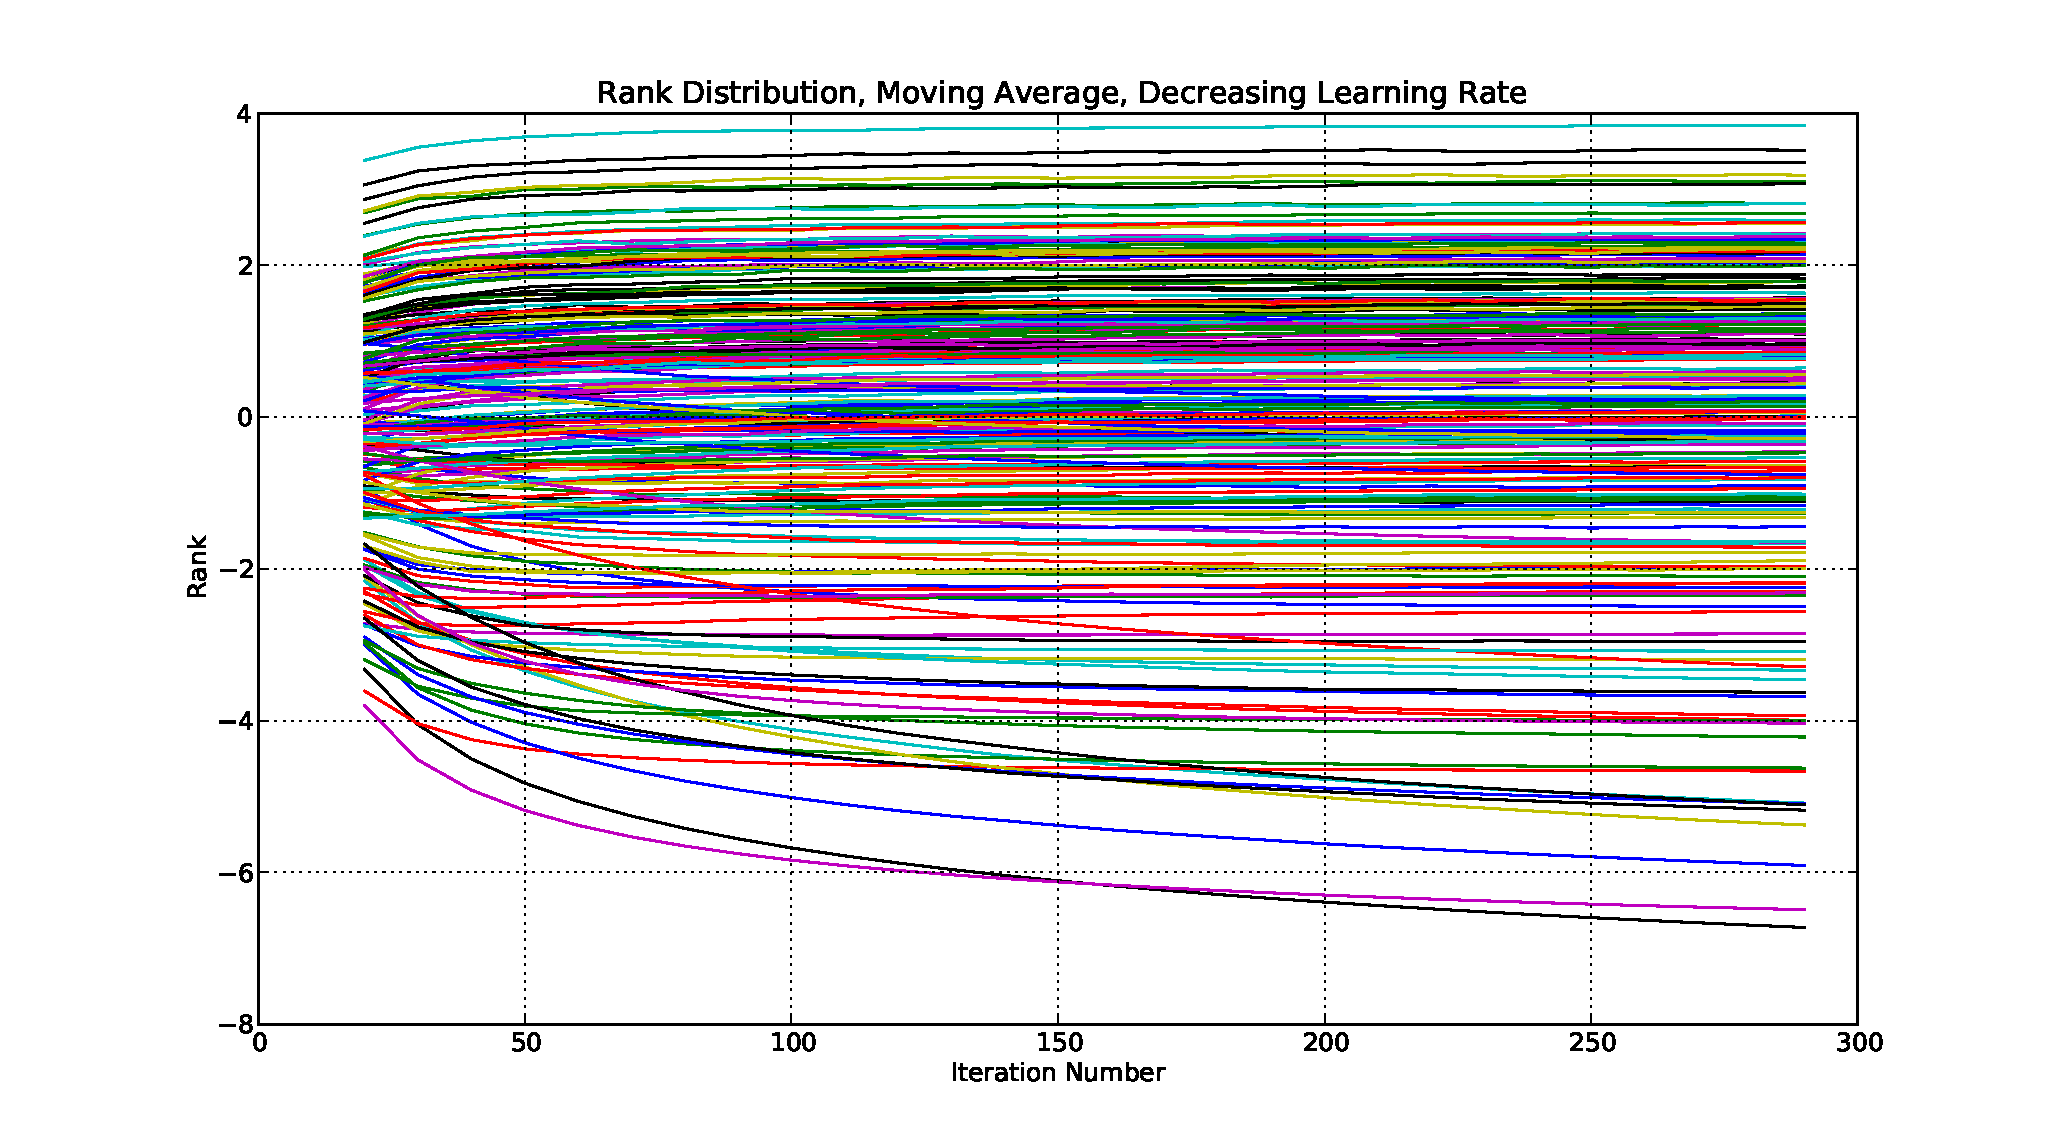
\includegraphics[width=0.45\linewidth]{RankMovAvgLearn300.pdf}
        \label{fig:ranklearn300}
        }
    \end{center}
    \caption{Convergence of ranks}
    \label{fig:rankconvergence}
\end{figure}

\begin{table}
    \centering
    \subfloat[Iteration Count ($\gamma$ = 1.5)]{
        \begin{tabular}{r|r|r|r}
            Iterations & All-or-Nothing Score & 80/20 Score & PDF Score \\
            \hline
            50  & 0.5683 & 0.5020 & 0.4814 \\
            100 & 0.5719 & 0.5048 & 0.4805 \\
            150 & 0.5717 & 0.5046 & 0.4816 \\
            200 & 0.5710 & 0.5041 & 0.4811 \\
            250 & 0.5708 & 0.5039 & 0.4816 \\
            350 & 0.5690 & 0.5025 & 0.4811
        \end{tabular}
        \label{tab:iter}
    }
    \subfloat[Factor ($\gamma$) (Iteration Count = 150]{
        \begin{tabular}{r|r|r|r}
            Factor ($\gamma$) & All-or-Nothing Score & 80/20 Score & PDF Score \\
            \hline
            0    & 0.5679 & 0.5016 & 0.4769 \\
            0.5  & 0.5692 & 0.5027 & 0.4780 \\
            1    & 0.5708 & 0.5040 & 0.4798 \\
            1.5  & 0.5714 & 0.5044 & 0.4814 \\
            2    & 0.5679 & 0.5016 & 0.4800 \\
            2.5  & 0.5619 & 0.4968 & 0.4824 \\
            3    & 0.5588 & 0.4943 & 0.4765
        \end{tabular}
        \label{tab:factor}
    }\\
    \subfloat[Bin Width (Iteration Count = 150, $\gamma$ = 1.5)]{
        \begin{tabular}{r|r|r|r}
            Bin Width & All-or-Nothing Score & 80/20 Score & PDF Score \\
            \hline
            0.01 & 0.5703 & 0.5039 & 0.4600 \\
            0.1  & 0.5714 & 0.5060 & 0.4730 \\
            0.25 & 0.5714 & 0.5050 & 0.4815 \\
            0.5  & 0.5580 & 0.4936 & 0.4971 \\
            1    & 0.5579 & 0.4936 & 0.5110 \\
            2    & 0.5579 & 0.4936 & 0.5197
        \end{tabular}
        \label{tab:binwidth}
    }
    \caption{Cross-validation results for a wide range of model parameters and scoring schemes illustrates that increasing complexity is not always the best choice. In this case, we find that the number of iterations used has a relatively low impact on predictive power. We also see that the All-Or-Nothing approach to prediction out performs the more conservative methods in every single test.}
    \label{tab:performance}
\end{table}

\subsection{Na\"ive Model}
As an additional test, we implemented the simplest data-based model possible. We refer to this as the Na\"ive Counting model. Applying the model consists of simply counting all matches between the two teams, and generating probability of win, tie, or loss directly from the counts.
\begin{align*}
    P(win) = \frac{wins}{matches}, \qquad
    P(tie) = \frac{ties}{matches}, \qquad
    P(loss) = \frac{losses}{matches}
\end{align*}
Under this model, we find that the overall score remains around 0.38, with a maximum of 0.4. Curiously, using the actual data-based likelihoods outperform the All-Or-Nothing and 80-20 models. In all cases, this model under-performs compared to our original model, which is expected. This model does not take many factors into account, such as home-team advantage. Additionally, the training method used greatly reduces the effective amount of training data available.
\begin{table}
    \centering
    \begin{tabular}{r|r|r}
        All-or-Nothing Score & 80/20 Score & PDF Score \\
        \hline
        0.3835 & 0.3561 & 0.4030 \\
    \end{tabular}
    \caption{Scores for the Na\"ive Counting model. In this case, the resulting PDFs prove to be more accurate predictors than in the other two models.}
    \label{tab:naive}
\end{table}


\section{Conclusion}
We find that our model performs reasonably well, and significantly better than the expected score of 0.33 for random selection. However, we also are somewhat disappointed to note that it is perhaps too fine-grained for this particular application and so many of the more complicated features provide little to no statistical benefit. For example, we use a smart, adaptive convergence test to determine when it is appropriate to terminate the ranking algorithm and begin prediction, but experimentation shows that simply choosing 100 or so iterations is sufficient, even if a few teams are slightly departed from their ``true'' rank.

We also find that the All-Or-Nothing approach to scoring, where we take the PDF as simply an indicator for which outcome we should invest 100\% confidence in, to be the most successful method for maximizing the score. While this was initially unintuitive, we are able to explain it mathematically. Further, we find that the PDF generation is still necessary for determining which outcome to select.

%%% BIBLIOGRAPHY %%%
\begin{thebibliography}{7}
\bibitem{FIFAranking}
  http://www.fifa.com/worldranking/rankingtable/index.html
\bibitem{FIFAcalc}
  http://www.fifa.com/worldranking/procedureandschedule/menprocedure/index.html
\bibitem{Sismanis}
  Y. Sismanis, \emph{How I won the "Chess Ratings - Elo vs the Rest of the World" Competition}, arXiv:1012.4571v1, 2010.
\end{thebibliography}

\end{document}
